

minepump

elevator

\subsection{Random games}
We can create a random variability parity game by creating a random parity game and creating sets of configurations that guard the edges. For these sets we need to consider two factors: how large are the sets guarding the edges and how are they created.

The guard sets in the minepump and elevator games have a very specific distribution where on average $99\%$ of the sets admit either $100\%$ or $50\%$ of the configurations. An edge requiring the presence or absence of a specific feature results in a set admitting $50\%$, this explains the distribution. The average edge in the examples admits $92\%$ of the configurations. 

We will use $\lambda$ to denote the average size of guard sets in VPGs. We will create random games with a specific $\lambda$, we do this by using a probabilistic distribution ranging from $0$ to $1$ to determine the size of every guard set. Such a distribution will have a mean equal to $\lambda$. We will consider two distributions:
\begin{itemize}
	\item A modified Bernoulli distribution; in a Bernoulli distribution there is a probability of $p$ to get an outcome of $1$ and a probability of $1-p$ to get an outcome of $0$. We modify this such that there is a probability of $p$ to get $1$ and a probability of $1-p$ to get $0.5$. This gives a mean of $1p + 0.5(1-p) = 0.5p + 0.5$. So to get a mean of $\lambda$ we choose $p = 2\lambda - 1$. Note that we can't use this distribution when $\lambda < 0.5$ because $p$ becomes larger than $1$.
	\item A beta distribution; a beta distribution ranges from $0$ to $1$ and is curved such that it has a specific mean. The beta distribution has two parameters: $\alpha$ and $\beta$ and a mean of $\frac{\alpha}{\alpha+\beta}$. We will pick $\beta=1$ and $\alpha = \frac{\lambda\beta}{1-\lambda}$ to get a mean of $\lambda$.
\end{itemize}
Figures \ref{fig:dist_lambda50}, \ref{fig:dist_lambda75} and \ref{fig:dist_lambda90} show the shapes of the distribution for different values for $\lambda$.
\begin{figure}[H]
	\centering
	\begin{subfigure}{.5\textwidth}
		\centering
		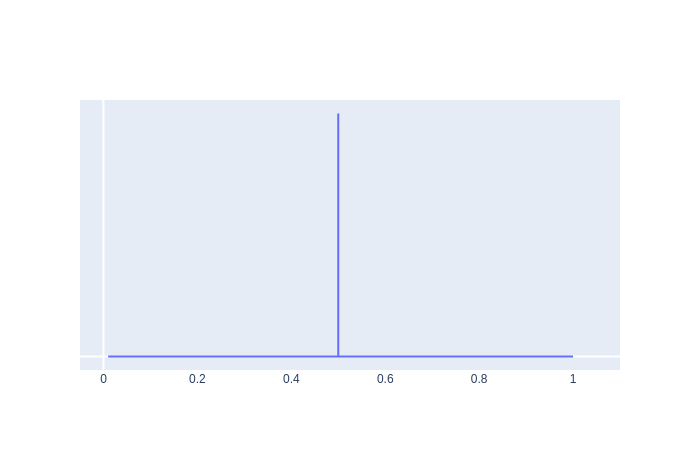
\includegraphics[width=\linewidth]{Dists/Bernoulli50.png}
		\caption{Modified Bernoulli distribution with $p=0$}
	\end{subfigure}%
	\begin{subfigure}{.5\textwidth}
		\centering
		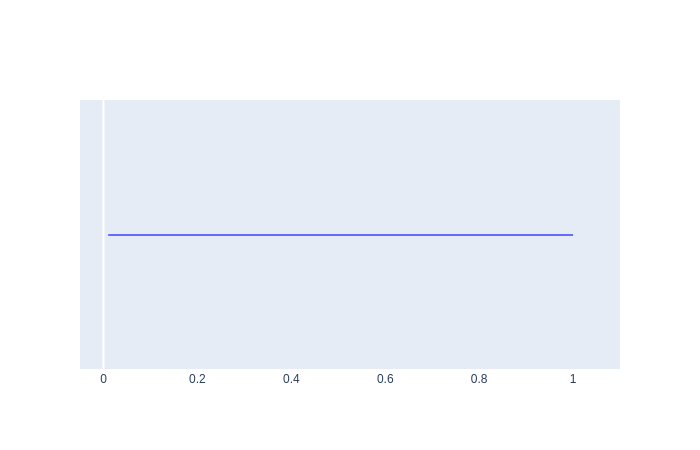
\includegraphics[width=\linewidth]{Dists/Beta50.png}
		\caption{Beta distribution with $\beta=1$ and $\alpha=1$}
	\end{subfigure}
	\caption{Edge guard size distribution for $\lambda = 0.5$}
	\label{fig:dist_lambda50}
\end{figure}%
\begin{figure}[H]
\centering
\begin{subfigure}{.5\textwidth}
	\centering
	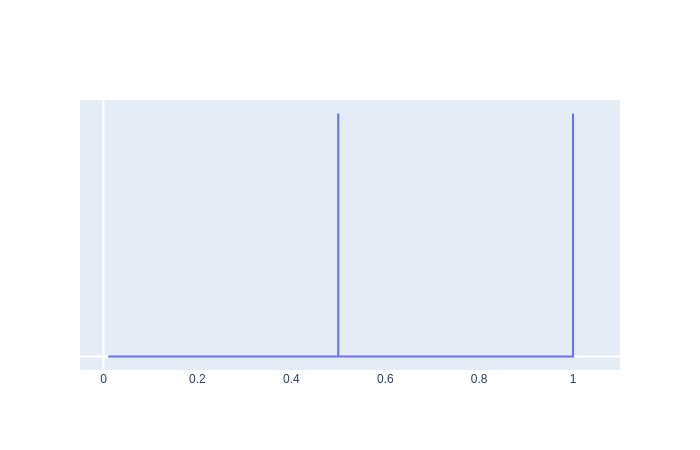
\includegraphics[width=\linewidth]{Dists/Bernoulli75.png}
	\caption{Modified Bernoulli distribution with $p=0.5$}
\end{subfigure}%
\begin{subfigure}{.5\textwidth}
	\centering
	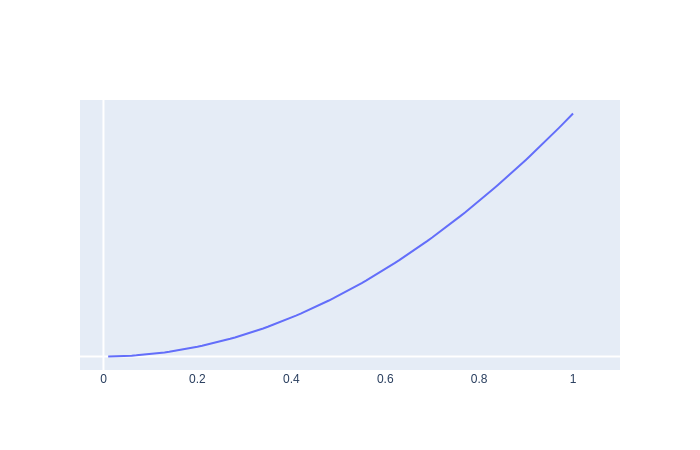
\includegraphics[width=\linewidth]{Dists/Beta75.png}
	\caption{Beta distribution with $\beta=1$ and $\alpha=3$}
\end{subfigure}
\caption{Edge guard size distribution for $\lambda = 0.75$}
\label{fig:dist_lambda75}
\end{figure}%
\begin{figure}[H]
\centering
\begin{subfigure}{.5\textwidth}
	\centering
	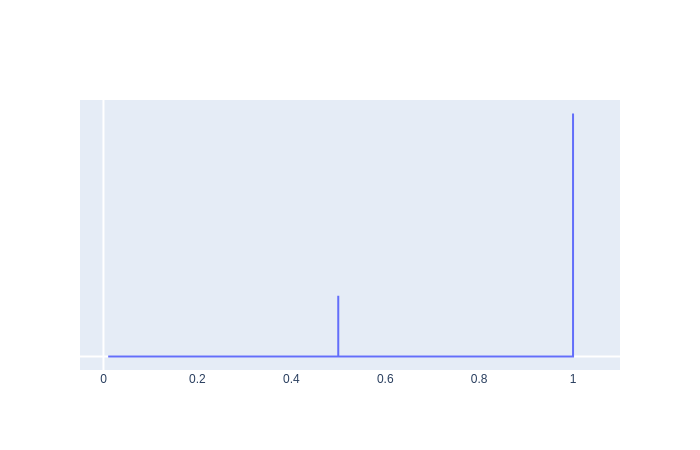
\includegraphics[width=\linewidth]{Dists/Bernoulli90.png}
	\caption{Modified Bernoulli distribution with $p=0.8$}
\end{subfigure}%
\begin{subfigure}{.5\textwidth}
	\centering
	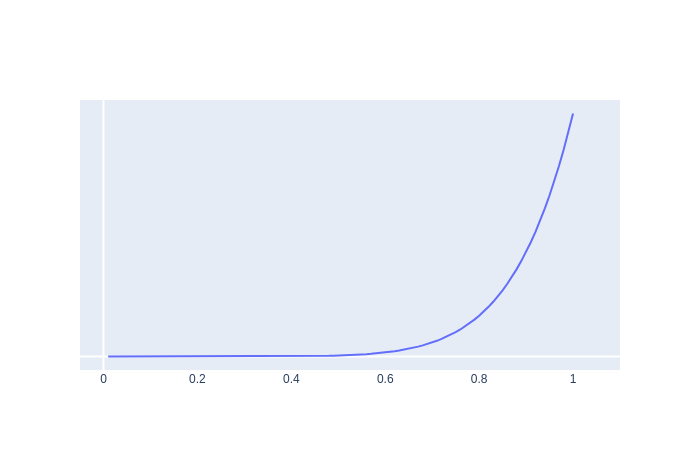
\includegraphics[width=\linewidth]{Dists/Beta90.png}
	\caption{Beta distribution with $\beta=1$ and $\alpha=9$}
\end{subfigure}
\caption{Edge guard size distribution for $\lambda = 0.9$}
\label{fig:dist_lambda90}
\end{figure}

Next we need to consider how the set of configuration is created. We can simply create a random set of configurations without any notion of features, we call this a \textit{configuration based} approach. Alternatively we can use a \textit{feature based} approach where we create sets by looking at features. Consider features $f_0, \dots, f_m$, we can create a boolean function that is the disjunction of $k$ features where every feature in the disjunction has probability $0.5$ of being negated.  For example when using $k=3$ and $m=5$ we might get boolean formula $f_1 \vee \neg f_2 \vee \neg f_4$. Such a boolean formula corresponds to a set of configurations of size $2^{m-k}$ and a relative size $\frac{2^{m-k}}{2^m} = 2^{-k}$, so when creating a set with relative size $r$ we choose $k = \min(m, \lfloor -\log_2{r} \rfloor)$. When using a feature based approach we can only create sets that have a relative size of $\frac{1}{2^i}$ for some $i \in \mathbb{N}$.

We can create 4 types of games:
\begin{enumerate}
	\item Bernoulli distributed and feature based. These games are most similar to the model verification games.
	\item Bernoulli distributed and configuration based. These games do have the characteristics of a model verification game in terms of set size but have unstructured sets guarding the edges. Furthermore with a configuration based approach less guard sets will be identical than with a feature based approach.
	\item Beta distributed and configuration based. These games are most different from the model verification games.
	\item Beta distributed and feature based. Games created in this way don't have the average relative set size of $\lambda$ because the feature based approach can only create sets of size $\frac{1}{2^i}$ for any $\lambda \geq \frac{1}{2}$ all the sets have either relative size $\frac{1}{2}$ or $1$, so effectively this creates the same games as using the Bernoulli distribution only with an incorrect average relative set size. Therefore we will not consider this category of games.
\end{enumerate}
\subsection{Categories}
For random games of type 1,2 and 3 we create 50 games: game 50 to game 99, where game $i$ has $\lambda=\frac{i}{100}$ and a random number of features, nodes, edges and maximum priority.

Furthermore we create 48 games to evaluate how the algorithm scales when the number of features becomes larger. For every $i \in [2,12]$ we create a random games $i$a, $i$b, $i$c and $i$d of type 1 with $\lambda=0.92$, $i$ features and a random number of nodes, edges and maximum priority.